\subsection{Etude de l'user story}

	Le Fronting Digital est avant tout une application destiné aux banquiers afin de leur permettre de gérer plus efficacement et facilement leurs entrées en relation. Or, lors d'une ouverture de compte ou d'une souscription à une assurance vie il est obligatoire de fournir certains documents comme une pièce d'identité, un relevé d'identité bancaire ou encore un justificatif de domicile. Ici, ces documents sont appelés "pièces justificatives" et ont fait l'objet d'une user story sur laquelle j'ai travaillé de manière autonome, coinjointement avec un autre stagiaire. \\
	
	Le contenu de cette story concernait la mise en place d'un nouvel écran sur l'application depuis lequel il est possible d'uploader/downloader des pièces justificatives. Les pièces obligatoires qui doivent être fournies par le futur client de la banque dépendent de ses données personnelles. Par exemple, un client personne physique mineur ne fournira pas les même pièces qu'un client personne morale. Ainsi, le nouvel écran doit pré-afficher la liste des pièces obligatoires en la calculant au préalable à partir des données saisies par le banquier. La story mettait à notre disposition une matrice définissant l'ensemble des règles de gestion permettant de déterminer, à partir des données, si une pièce était obligatoire ou non. De plus, l'écran doit aussi proposer un menu déroulant permettant de choisir n'importe quel type de pièce afin de l'ajouter manuellement à la liste. Les pièces ajoutées de cette manière sont facultatives et doivent être affichées d'une couleur différente. Il est possible de retrouver en annexe \ref{frontingDigitalPJ} une maquette illustrant ce nouvel écran. \\

	Comme nous l'avons expliqué dans la partie \ref{deroulementSprint}, la première étape pour l'équipe de développement consiste à prendre connaissance de l'user story afin de la découper en tâches unitaires. Ici, nous avons fait le choix de créer 5 tâches qui sont les suivantes :
	
	\subsubsection{Composant pièce justificative}
	Le composant "pièce justificative" est un composant Angular représentant la brique qui contient tous les éléments et options d'une pièce justificative à savoir :
	\begin{itemize}
		\item Le fichier
		\item La date de fin de validité
		\item L'accord dérogatoire
		\item La date d'upload du fichier
		\item La possibilité de supprimer la pièce
		\item La possibilité de visualiser la pièce (ou la télécharger si elle ne peut être visualiser sur le navigateur)
	\end{itemize}
	Cette brique est représentée par un rectangle rouge sur l'annexe \ref{frontingDigitalPJ}
	
	\subsubsection{Composant écran pièce justificative}
	Ce composant est l'écran sur lequel sont affichées les pièces justificatives sous la forme d'une liste dont les éléments sont les composants décrits précédemment. Celui-ci pré-remplie la liste avec les pièces définies comme étant obligatoires. Ainsi, le banquier aura un rapide aperçu des pièces qu'il doit demander à son client et n'aura qu'à uploader les fichiers pour compléter la liste. De plus, un menu déroulant doit être présent, permettant de rajouter des pièces manuellement à la liste, dites facultatives qui apparaissent d'une couleur différente. En outre, le service d'appel front devra être créé afin de pouvoir communiquer avec l'API et consommer les web services. En outre, l'écran doit être accessible depuis la barre de navigation principale de l'application et un compteur indiquant le nombre de pièces obligatoires fournies/totales (par exemple 2/5) doit figurer au-dessus de la barre.
	
	\subsubsection{Référentiel}
	Dans notre application apparait un certain nombre de données métiers constantes comme la liste des pays pour un client, la liste des départements pour la France ou encore la liste des formes juridiques pour une entreprise. Pour toutes ces listes de données un endpoint est ajouté et un service appelé \textit{référentiel} est créé. Ainsi, il est possible de les obtenir de manière simple depuis le front en consommant le service adéquat. Si les métiers ont le besoin de modifier les valeurs, il suffit d'apporter une simple modification rapide et cela permet de garder un code structuré et clair. Dans notre cas, un référentiel devait être créé afin de référencer tous les types de pièces justificatives prises en charge par la banque (carte d'identité, justificatif de domicile, etc... pour un total de 41 différentes).	
	
	\subsubsection{Backend}
	Comme son nom l'indique, cette tâche consiste à développer les services backend destinés à alimenter notre frontend. Cela implique la création du contrôleur et de tous les endpoints, le service dédié ainsi que le modèle permettant de gérer les pièces justificatives. De plus, cela inclut le paramétrage pour la limite de taille des fichiers à uploader ainsi que la validation des données reçues.
	
	\subsubsection{Moteur de calcul}
	Nous avons dit plus haut que l'écran des pièces dévait pré-afficher la liste des pièces obligatoires. Or, le fait qu'une pièce soit obligatoire ou non dépend des données personnelles du client de la banque. Ainsi, le moteur de calcul doit prendre en compte l'ensemble des règles de gestion métiers ainsi que les données entrées jusqu'à présent par le banquier dans l'application afin de définir la liste des pièces obligatoires puis la transmettre au composant écran. \\
	
	Comme je l'ai dit plus haut, j'ai travaillé sur cette story avec un autre stagiaire. Ainsi, nous nous sommes séparé les tâches avant de commencer c'est pourquoi je me suis plutôt occupé de la partie backend et lui de la partie frontend. Ce découpage permettait d'avancer en parallèle sans problèmes. \\
	
\subsection{Sprint planning}
	Après avoir étudier l'user story et définie les différentes tâches à réaliser, une réunion de type sprint planning a eu lieu afin de définir la charge de travail pour effectuer chacune d'entre elles. Au cours de cette réunion nous avons voté et la charge a été réparti de la manière suivante :
	
\begin{table}[h!]
	\center
	\begin{tabular}{| c | c |}
     \hline
     Tâche & Charge (jour) \\ \hline
     Composant pièce justificative & 3.75\\ \hline
     Composant écran justificatifs & 3.75\\ \hline
     Backend & 2.25\\ \hline
     Référentiel & 1.5\\ \hline
     Moteur de calcul & 9.75\\
     \hline
	\end{tabular}
	\caption{Sprint planning pièces justificatives}
	\label{sprintPlanningPJ}
\end{table}

	Une fois le sprint planning terminé nous avons pu passer à la conception de nos tâches respectives ainsi qu'à la phase de développement.

\subsection{Conception backend}

	\subsubsection{Endpoints - couche controller}

	Dans un premier temps, j'ai commencé par définir les différents cas d'utilisation possible d'un banquier qui utiliserait l'écran des pièces justificatives. Il est possible d'observer ces cas sur le diagramme figure \ref{useCasePJ}.

\begin{figure}[h!]
	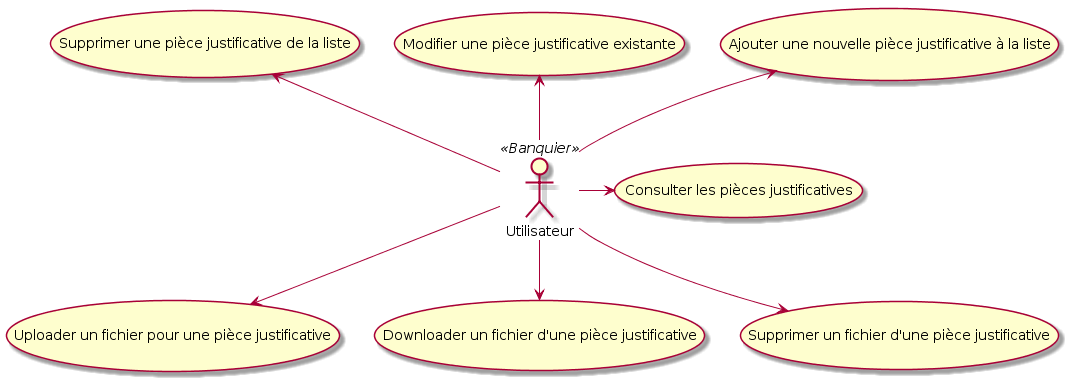
\includegraphics[scale=0.50]{images/travailBP1818/piecesJustif/useCasePJ.png}
	\centering
	\caption{Cas d'utilisation}
	\label{useCasePJ}
\end{figure}

	Pour chacun de ces derniers j'ai décidé de mettre en place un service permettant de répondre au besoin qu'il définissait. J'ai ainsi pu procéder à la création du contrôleur ainsi que des endpoints permettant d'exposer les services répondant aux cas d'utilisation. Pour cela, il a fallu déterminer les méthodes HTTP et l'url associée que notre client pourra intéroger en essayant de rester RESTful. Le tableau suivant décrit les endpoints ainsi créés :
	
\begin{table}[h!]
	\center
	\begin{tabular}{| c | c | c |}
     \hline
     Cas d'utilisation & Méthode HTTP & URL \\ \hline
     Obtenir pièces justificatives & GET & /justificatifs/{idForm}\\ \hline
     Créer pièce justificative & POST & /justificatifs/{idForm}/justificatif\\ \hline
     Modifier pièce justificatives & PUT & /justificatifs/{idForm}/justificatif\\ \hline
     Supprimer pièce justificative & DELETE & /justificatifs/{idForm}/justificatif\\ \hline
     Downloader fichier & GET & /{idForm}/fichier\\ \hline
     Uploader fichier & POST & /{idForm}/fichier\\ \hline
     Supprimer fichier & DELETE & /{idForm}/fichier\\ \hline
	\end{tabular}
	\caption{Sprint planning pièces justificatives}
	\label{sprintPlanningPJ}
\end{table}

	En outre, j'ai créé un endpoint supplémentaire que j'ai placé dans le contrôleur \textit{ReferentielController} dédié aux référentiels. Celui-ci permet d'accéder au référentiel des pièces justificatives et donc d'obtenir la liste des types de pièces qu'il est possible d'utiliser dans l'application.

	\subsubsection{Modèle - couche domain}
	
	Comme nous l'avons vu dans la partie \ref{archiBP1818}, nous avons recours à Couchbase pour notre base de données de type NoSQL. Ainsi, toutes les données sont enregistrées sous la forme de documents au format JSON. Dans notre cas, nous avons généralement un document par formulaire dont le nom est constitué de l'id du client et d'un préfixe permettant d'identifier rapidement le formulaire. Par exemple, nous avons un écran sur lequel il est possible de spécifier les données personnelles du client. Le formulaire est sauvegardé dans un document portant le nom \textit{TIERS\_10001} pour le client d'id 10001. Nous avons un écran déroulant une série de questions sur les patrimoines et revenus du client. Le formulaire regroupe les réponses à toutes les questions et est sauvegardé dans le document \textit{PAT\_10001}, toujours pour le client d'id 10001. Ainsi, dans le cas des pièces justificatives j'ai décidé de sauvegarder l'ensemble du formulaire contenant les pièces dans un nouveau document dont le nom serait \textit{JUST\_ID}. \\
	
	Une fois cela définit, il fallait déterminer quelles données devaient être persistées ainsi que leur structure. J'ai donc commencé par définir le modèle qui serait utilisé en étudiant plus en profondeur l'user story afin de relever toutes les informations à persister. Ce modèle peut être représenter par le diagramme de classe figure \ref{modelePJ}.	
	
\begin{figure}[h!]
	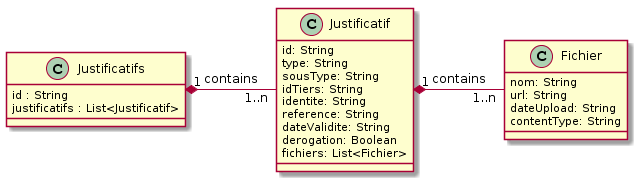
\includegraphics[scale=0.7]{images/travailBP1818/piecesJustif/modelePJ.png}
	\centering
	\caption{Modèle des pièces justificatives}
	\label{modelePJ}
\end{figure}

	La classe \textit{Fichier} représente un fichier uploadé par le banquier et contient ses informations comme son nom, l'url indiquant à quel endroit est enregistré le fichier, la date à laquelle il a été enregistré et son content-type. Celui-ci est une en-tête permettant d'indiquer le type MIME d'une ressource, nécessaire dans notre cas pour visualiser le fichier dans le navigateur. \\
	
	Ensuite, la classe \textit{Justificatif} représente une pièce justificative et toutes les informations qui lui sont associées comme le type ou la date de validité. Elle contient aussi l'id du tiers ("idTiers") à qui elle appartient afin de pouvoir l'identifier ainsi que son identité ("identite") afin de pouvoir afficher le nom de son propriétaire côté frontend (par exemple carte d'identité de M. Jean Dupont). En outre, cette classe contient une liste de fichier ("fichiers") contenant tous les fichiers uploadés pour la pièce justificative (par exemple pour une carte d'identité il peut y avoir deux fichiers : une image pour le recto et une pour le verso). \\
	
	Enfin, la classe \textit{Justificatifs} contenant l'id du document au format JUST\_ID ainsi qu'une liste de pièces justificatives ("justificatifs"). \\
	
	J'ai pu implémenter ce modèle en Java en créant des Beans côté backend. Nous utilisons actuellement Maven comme outil de gestion et d'automatisation de production de logiciel. Nous avons configuré un plugin Maven, nommé \textit{Typescript Generator}, permettant de générer le modèle côté frontend. En effet, une fois le modèle créé côté backend, il suffit de relancer un build Maven afin que ce plugin génère le code Typescript à partir du code Java. Un fichier est créé contenant toutes les interfaces typescript obtenues à partir des Beans java. Cela nous permet d'assurer la cohérence entre nos modèles back et front et nous permet de gagner beaucoup de temps en nous évitant de réécrire une seconde fois le modèle.
	  
	
	\subsubsection{Communication avec Couchbase - couche repository}
	
	Le modèle étant défini, il fallait maintenant mettre en place la communication avec Couchbase afin de persister les données ou les récupérer. Pour cela, j'ai créé un repository pour les pièces justificatives. Comme nous l'avons vu plus haut, il s'agit d'une interface facilitant grandement l'utilisation de requêtes vers notre base de données. Le schéma figure \ref{repository} illustre le fonctionnement du repository des pièces justificatives. \\
	
	J'ai donc créé JustificatifsRepository et fait en sorte que la classe \textit{Justificatifs} implémente l'interface IdentifiableDocument. Pour cette user story aucune autre requête que celles fournies était nécessaire donc aucun développement supplémentaire était requis. \\

\begin{figure}[h!]
	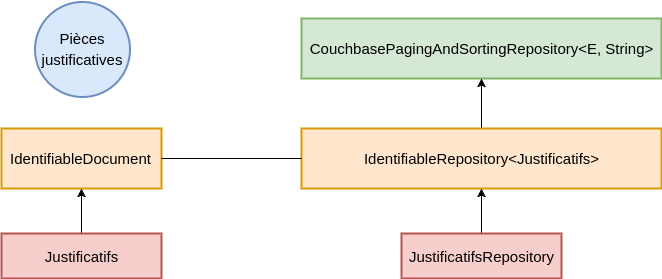
\includegraphics[scale=0.55]{images/travailBP1818/piecesJustif/repositoryPJ.png}
	\centering
	\caption{Repository pièces justificatives}
	\label{repositoryPJ}
\end{figure}
		
	\subsubsection{Service - couche service}
	
	A ce stade, les cas d'utilisation étaient connus, le modèle défini, la communication avec Couchbase établie et les endpoints exposant les services prêts. La prochaine étape consistait à effectivement développer les services permettant de répondre aux différents besoins identifiés sur le diagramme figure \ref{useCasePJ}.
	
\begin{table}[h!]
	\center
	\begin{tabular}{| c | c |}
     \hline
     Services & Description \\ \hline
     findJustificatifs & Permet de retourner le formulaire JUST\_ID contenant toutes les pièces \\ \hline
     createPiece & Permet de créer pièce justificative en l'ajoutant au formulaire \\ \hline
     updatePiece & Permet de mettre à jour une pièce justificative du formulaire \\ \hline
     deletePiece & Permet de supprimer une pièce justificative en la supprimant du formulaire \\ \hline
     uploadFile & Permet d'uploader un fichier \\ \hline
     downloadFile & Permet de downloader un fichier \\ \hline
     deleteFile & Permet de supprimer un fichier\\ \hline
	\end{tabular}
	\caption{Services pièces justificatives}
	\label{servicesPJ}
\end{table}

	Comme nous l'avons expliqué, l'écran des pièces justificatives doit présenter la liste des pièces obligatoires obtenu par le biais du moteur de calcul. Pour chacune de ces pièces il est possible d'ajouter un ou plusieurs fichiers en appelant le service uploadFile. Comme il est possible de l'observer sur le diagramme figure \ref{seqSave} et à la demande des métiers, une pièce est sauvegardée si et seulement si elle possède un fichier. Dans le cas contraire la pièce n'est pas ajoutée au formulaire qui sera envoyé au back par la suite et ne sera donc pas sauvegardée. En effet, si une pièce obligatoire ne possède pas de fichier elle sera simplement ajoutée par le moteur de calcul implémenté côté front. Concernant les pièces facultatives, il est logique qu'elles ne soient pas sauvegardées si aucun fichier n'est ajouté. A chaque fois qu'un fichier est ajouté à une pièce, une requête POST est envoyée via le service createPiece afin de créer la pièce côté back s'il s'agit de son premier fichier sinon une requête PUT est envoyée via le service updatePiece afin de mettre à jour le formulaire des pièces justificatives. \\

\begin{figure}[h!]
	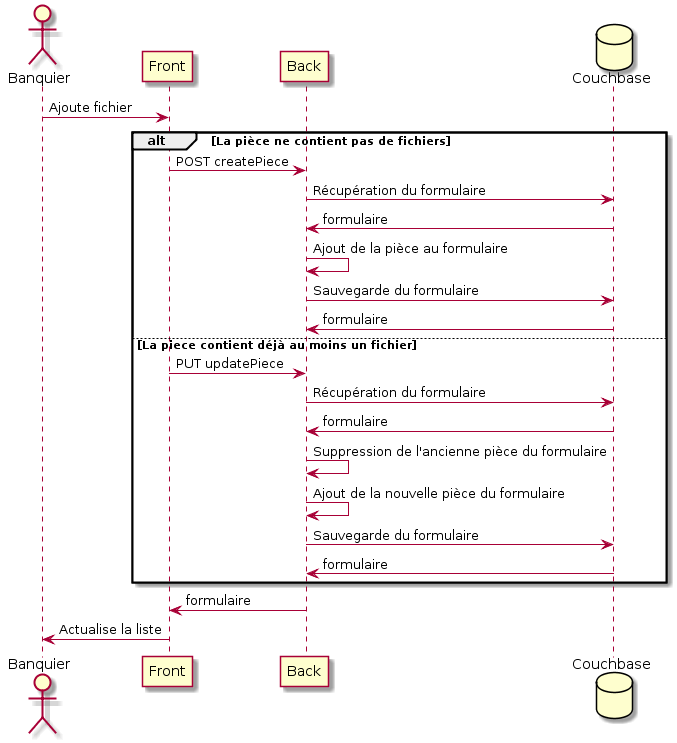
\includegraphics[scale=0.55]{images/travailBP1818/piecesJustif/seqSave.png}
	\centering
	\caption{Sauvegarde des pièces justificatives}
	\label{seqSave}
\end{figure}

	Ensuite, lorsque l'utilisateur souhaite accéder à l'écran des pièces justificatives, le moteur de calcul fourni la liste des pièces obligatoires pendant qu'une requête est envoyée côté back via le service findJustificatifs pour récupérer le formulaire contenant toutes les pièces sauvegardées de manière asynchrone. Une fois les deux listes obtenues, elles sont mergées en une liste finale afin d'éliminer les doublons qui sera affichée sur l'écran. Par exemple, le moteur peut indiquer que la pièce "carte d'identité" est obligatoire. Si les fichier de la carte d'identité du titulaire du compte ont bien été ajouté et sauvegardé alors lors du merge de la liste du moteur et de la liste du back, seule la pièce "carte d'identité" du back sera gardée. Le diagramme de séquence réalisé pour ce cas figure \ref{seqGet} illustre ce principe. En sauvegardant et récupérant les pièces de cette manière nous pouvons maintenir la cohérence des données et limiter le nombre de requêtes envoyées à notre backend. \\
	
	Les autres services comme le téléchargement de fichiers ou la suppression de pièces n'ont pas nécessité de diagrammes et sont utilisés simplement par clic sur un bouton. \\

\begin{figure}[h!]
	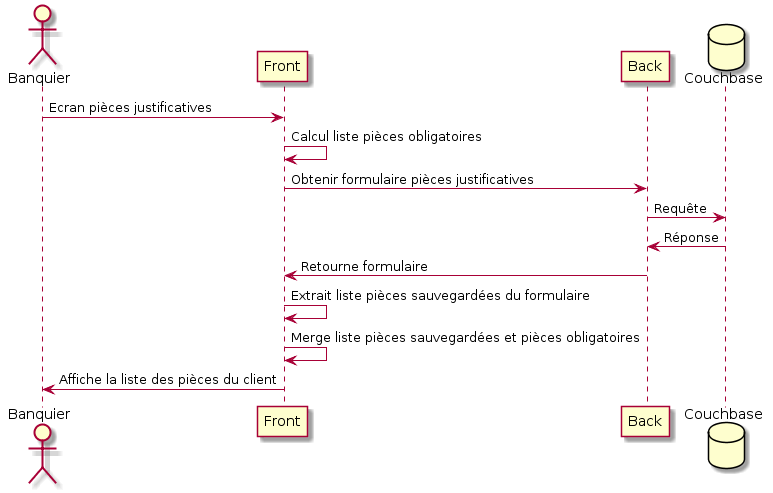
\includegraphics[scale=0.55]{images/travailBP1818/piecesJustif/seqGet.png}
	\centering
	\caption{Affichage des pièces justificatives}
	\label{seqGet}
\end{figure}

\subsection{Conception frontend}
	
	Pour la partie frontend je me suis chargé de mettre en place le moteur de calcul permettant de fournir la liste des pièces obligatoires pour un client de la banque. Pour cela, j'ai mis en place un service uniquement dédié à ce moteur. L'user story contenait une matrice listant toutes les pièces justificatives acceptées par la banque ainsi que les règles de gestion métiers indiquant si la pièce était obligatoire ou non. Que le client de la banque soit une personne physique ou une personne morale, ces règles n'étaient basées que sur les données personnelles de ce client. De ce fait, le service du moteur ne nécessitait que le formulaire des données personnelles dans le but de fournir la liste des pièces obligatoires. \\
	
	Comme je l'ai expliqué dans la partie \ref{frontendArchi}, nous avons mis en place différents resolver car nous avons parfois le besoin de charger certaines données avant l'initialisation d'un composant. Ainis, ici, j'ai utilisé un resolver dont l'objectif est de récupérer le formulaire contenant les données personnelles du client en intérogeant notre backend. Or, calculer la liste des pièces obligatoires ne suffit pas. En effet, il faut aussi afficher les pièces sauvegardées qui auraient déjà été ajoutées par le banquier en évitant les doublons. \\
	
	Par exemple, admettons que le moteur déclare que la pièce d'identité est obligatoire pour un client. Le banquier upload deux fichiers pour cette pièce (recto et verso de la carte d'identité du client en question). Comme nous l'avons vu, lorsqu'une pièce se voit attribuer un fichier, une requête PUT est envoyée côté back et la pièce est persistée sur Couchbase. Lorsque le banquier se rend à nouveau sur l'écran des pièces justificatives sans faire d'autres modifications sur l'application, le moteur déclarera toujours que la pièce d'identité est obligatoire. Or, cette dernière ayant déjà été complétée, il faut afficher la pièce sauvegardée déjà remplie issue de Couchbase et non pas celle issue du moteur qui est vide. \\
	
	Pour cette raison j'ai dû avoir recours à un second resolver permettant de récupérer le formulaire contant toutes les pièces sauvegardées sur Couchbase. Une fois les formulaires obtenus, ceux-ci sont envoyés au composant qui est alors initialisé. Lors de cette initialisation, le service du moteur de calcul est obtenu par injection de dépendance et calcule, dans un premier temps, la liste des pièces obligatoires puis merge cette liste avec la liste des pièces sauvegardées afin d'éliminer les doublons avant de l'afficher. \\
	
	En outre, l'écran doit proposer un menu déroulant permettant au banquier d'ajouter manuellement n'importe quel type de pièce. La pièce ajoutée ainsi sera alors facultative et apparaitra d'une couleur différente. Cependant, comme nous l'avons vu, les types de pièces sont issus d'un référentiel créé au préalable. Ainsi, lors de l'initialisation du composant, il fallait aussi récupérer la liste des types de pièces depuis ce référentiel. J'ai ici pu tirer profit des possibilités offertes par Angular en matière de programmation asynchrone. En effet, pendant que le composant récupère la liste des pièces qui sera affichée dans le menu déroulant, celui-ci appelle le service du moteur de calcul en parallèle. Cela nous permet de gagner un peu en rapidité et de compenser le temps perdu par les resolvers.

\subsection{Résultats et perspectives}

	Une fois le développement des fonctionnalités terminée, j'ai pu passer au développement des différents tests unitaires dont l'objectif premier est d'éviter les régressions de l'application à mesure que le code évolu. Après cela, le projet partiel est passé en phase de qualification où certaines anomalies ont été relevées avant d'être livré au client. C'est alors qu'une sprint review a eu lieu suivie d'une réunion de sprint planning pour le prochain sprint. Lors de cette réunion, nous commençons par effectuer une rétrospective du sprint précédent. Pour le sprint des pièces justificatives nous avons obtenu les résultats présents sur le tableau \ref{retroPJ}.

\begin{table}[h!]
	\center
	\begin{tabular}{| c | c | c |}
     \hline
     Tâche & Charge prévue (jour) & Charge réelle (jour) \\ \hline
     Composant pièce justificative & 3.75 & 6\\ \hline
     Composant écran justificatifs & 3.75 & 5\\ \hline
     Backend & 2.25 & 5\\ \hline
     Référentiel & 1.5 & 1\\ \hline
     Moteur de calcul & 9.75 & 2\\
     \hline
	\end{tabular}
	\caption{Rétrospective pièces justificatives}
	\label{retroPJ}
\end{table}
	
	Comme on peut l'observer, sur ce sprint, la charge réelle est en grand désaccord avec la charge prévue. Cela est en partie dû à une mauvaise estimation de notre part. Par exemple, j'ai réalisé le moteur de calcul bien plus vite que prévu. Nous avions mal estimé la complexité de cette tâche, ce qui peut être causé soit par une mauvaise compréhension de cette dernière soit par une mauvaise étude de l'user story avant le sprint planning. Cette seconde raison n'est pas à rejeter, il est en effet fréquent que l'équipe de développement soit très occupée par manque de ressource et nous ne disposons parfois que peu de temps pour nous imprégner des stories avant le sprint planning. Ce problème sera désormais réglé puisque deux nouveaux développeurs sont attendus pour la fin juillet. \\
	
	Ensuite, je ne pense pas que la faute concerne uniquement une mauvaise estimation. Certes cette dernière était biaisée mais cette user story était la première que j'ai réalisé en autonomie depuis sa lecture à sa réalisation en passant par sa conception. Il est probable qu'il y ait eu un certain manque de recul de ma part, ce qui m'a obligé à retoucher plusieurs mon modèle et donc ma conception initiale. Afin de pallier cela, je me suis chargé d'effectuer certaines tâches de refactoring dans l'application comme la mise en place d'un système de cache dont je vais parler ci-dessous ainsi que des test sur des fonctionnalités qui n'étaient pas testées pendant quelques jours. Cela m'a permi d'avoir une bien meilleure vision de l'application en explorant les parties du code dont je n'avais jamais pris connaissance tout en permettant de sécuriser le code contre les régressions. \\
	
	Enfin, dernier point qui a été pour moi et mon tuteur le principal problème : le manque de communication. En effet, j'ai travaillé avec un autre stagiaire sur cette story. Je me suis chargé du backend, du référentiel et du moteur de calcul pendant que lui s'occupait des composants frontend. Or, celui-ci ignorait que nous possédions un plugin maven générant le modèle frontend à partir du modèle backend et a donc mis en place son propre modèle de son côté. Nous nous sommes rendus compte de cela un peu tard lorsque nous avons commencé à essayer d'intégrer nos travaux et il a donc fallu retoucher le modèle ce qui nous a fait perdre du temps. Aujourd'hui, nous avons une bien meilleure communication et lorsque qu'il est nécessaire de travailler à plusieurs sur une même user story en se séparant les tâches (par exemple un sur le backend et l'autre sur le frontend) nous nous concertons avant et nous parlons dès que le modèle doit évoluer afin que l'autre soit toujours au courant et puisse rester cohérent. \\

	J'ai ici pris le sprint des pièces justificatives en guide d'exemple dans le but d'illustrer l'étude des spécifications, la conception ainsi que la réalisation d'un sprint de manière générale. L'ensemble des sprints se déroule de cette manière sur des périodes de deux à trois semaines selon les conditions et la charge de travail. Je ne décrirais pas plus en profondeur les autres sprints puisque le principe reste le même. Cependant, au cours de ces derniers j'ai parfois été amené à effectuer certaines tâches s'écartant des user stories. Par exemple, nous travaillons le code de manière incrémentale se qui implique des changements et des évolutions. De plus, lors des sprint review nous tenons compte des remarques client c'est pourquoi j'ai parfois été amené à faire du refactoring sur certaines fonctionnalités. \\
	
	Lors de la création d'une personne physique, l'écran affiche une barre de navigation avec les différents onglets disponibles (voir annexe \ref{d1}). Au-dessus de la mention de chacun de ces onglets il faut afficher une "coche" permettant d'indiquer si les données sont bien remplies. L'affichage de la coche doit toujours être calculée, qu'importe l'onglet dans lequel on se trouve. Le calcul se fait à partir de la validité du formulaire présent dans l'onglet en question. Cela implique de récupérer \textbf{l'ensemble} de tous les formulaires à chaque fois que l'on navigue dans l'application ce qui représente un grand nombre de requête vers notre backend et a pour conséquence une baisse de performance. Ainsi, j'ai pu mettre en place un système de cache côté frontend afin de ne plus requêter sans cesse notre API. Il pourrait être intéressant de mettre en place un système de cache côté backend à l'aide de \textit{redis cache manager} afin de diminuer le nombre de requêtes vers Couchbase. \\
	
	De plus, lors de la réalisation de ce refactoring je me suis rendu compte qu'il pourrait être bénéfique de mettre en place du monitoring pour notre application. En effet, certains autres outils de la stack Netflix fournissent de très bons résultats pour cela. \textit{Zipkin} permet de traquer toutes les requêtes effectuées et donc de déceler certains problèmes de parallélisation issus de la programmation réactive. \textit{Hystrix} de son côté propose des dashboards permettant d'effectuer du monitoring et du suivi d'erreur. La gestion des requêtes à destination de notre backend serait simplifier de part l'utilsiation de ces outils. Néanmoins, la mise en place de ces derniers requiert du temps et la mobilisation de certaines ressources, ce que nous ne pouvons pas nous permettre en ce moment. Cependant, pour les projets semblables à venir chez Natixis dont BP1818 est une filiale, ils pourraient être mis en oeuvre dès le début du projet.